\section{Filtro de Kalman}

Uno de los requerimientos principales del proyecto es lograr implementar un sistema que permita estimar con mayor precisión la posición del robot dentro de su entorno, para lo cual propusimos utilizar un Filtro de Kalman. Este algoritmo combina datos de múltiples sensores considerando el ruido e incertidumbre inherente a las mediciones y los procesos asociados. \cite{negenborn2003robot}

Su funcionamiento se basa en dos etapas: una de predicción, que estima el próximo estado del sistema a partir del modelo cinemático del robot, y otra de actualización, que corrige dicha estimación en función de los datos reales obtenidos por los sensores. Esta integración la desarrollamos en Python y permitió al robot ajustar su trayectoria en tiempo real, compensando errores por deslizamiento o irregularidades del terreno y mejorar el desempeño.

\subsection{Estimación de posición y velocidad con Filtro de Kalman}
El robot, mientras realiza movimientos y trayectorias, reporta mediciones realizadas por el modelo cinemático y la odometría cada $500[ms]$ conteniendo una tupla como se muestra en la expresión \ref{ec:vector_velocidades}:

\begin{equation}
    [\Delta x, v_x, \Delta y, v_y] 
    \label{ec:vector_velocidades}
\end{equation}

Donde $\Delta x$ y $\Delta y$ representan las distancias de desplazamiento, y $v_x$ y $v_y$ las velocidades instantáneas promedio del robot, todas correspondientes a cada eje cartesiano durante el último intervalo de tiempo.

Al mismo tiempo, diseñamos el filtro de modo que registre velocidad y posición en los ejes $x$ e $y$ con la tupla \ref{ec:vector_velocidades_lineales}:

\begin{equation}
    [x, v_x, y, v_y]
    \label{ec:vector_velocidades_lineales}
\end{equation}

Representando $x$ e $y$ la posición absoluta en los ejes $x$ e $y$, mientras que $v_x$ y $v_y$ las velocidades en estos. Es importante que la entrada y salida del filtro sean del mismo formato, es decir, tenga como entrada y salida la tupla $[x, v_x, y, v_y]$. En este caso introducimos al filtro las mediciones acumuladas en distancia y las velocidades instantáneas en cada eje cartesiano. Por otra parte, el funcionamiento del Filtro de Kalman nos permite actualizar el estado por cada medición recibida del robot y calcular el vector de compensación según el estado estimado por el filtro.

El filtro de Kalman requiere el modelo matemático de nuestro sistema. Este se desarrolla en base a la ecuación de movimiento rectilíneo acelerado, por lo que para la posición y velocidad instantáneas se tienen las ecuaciones \ref{ec:posicion} y \ref{ec:velocidad}:

\begin{equation}
    x = x_0 + x_0 \Delta t + \frac{1}{2} a \Delta t^2
    \label{ec:posicion}
\end{equation}

\begin{equation}
    v_x = v_0 + a\Delta t
    \label{ec:velocidad}
\end{equation}

La secuencia de procesos a realizar cada vez que se recibe una medición del robot es la siguiente: \\

\begin{enumerate}
\item \textbf{Cálculo del Estado Predicho $X_{kp}$} \mbox{} \vspace{4pt}

Este término expone en donde debería estar el robot según el modelo ideal y la distancia entre muestras $\Delta t$. En base a lo anterior en forma matricial, tenemos que el estado predicho está dado por la ecuación \ref{ec:estado_predicho}:

\begin{equation}
    X_{kp} =
    \begin{bmatrix}
        x_{kp} \\ v_{kp} \\ 
    \end{bmatrix}
    =
    A \cdot X_{k-1} + B \cdot U_k + \omega_k
    \label{ec:estado_predicho}
\end{equation}

Las matrices $A$ y $B$ representan al modelo en base a las ecuaciones \ref{ec:posicion} y \ref{ec:velocidad}, mientras que $\omega_k$ representa algún ruido o perturbación presente en el proceso de cálculo del estado predicho \ref{ec:estado_predicho}. En nuestro caso lo consideramos despreciable, por lo que es nulo. Además, el vector $U_k$ se considera nulo dado que no llevamos registro de la aceleración del robot.

Donde:

\begin{equation}
    X_{k-1} = \begin{bmatrix} x_{k-1} \\ v_{k-1} \\ \end{bmatrix}
;
A = \begin{bmatrix}
    1 & \Delta t  \\
    0 & 1         \\
    \end{bmatrix} \\
;
B = \begin{bmatrix}
    \frac{1}{2} \Delta t^2 \\
    \Delta t               \\
    \end{bmatrix}          \\
\end{equation}

\begin{equation}
    U_k = \begin{bmatrix} a_0 \\ \end{bmatrix} \\
    ;
    \omega_k = \begin{bmatrix} 0 \\ 0 \\ \end{bmatrix}
\end{equation}

Entonces la ecuación para obtener el nuevo estado predicho es:

\begin{equation}
    X_{kp} = 
    \begin{bmatrix}
    1 & \Delta t  \\
    0 & 1         \\
    \end{bmatrix} \\
    \cdot \begin{bmatrix} x_{k-1} \\ v_{k-1} \\ \end{bmatrix}
    +
    \begin{bmatrix}
    \frac{1}{2} \Delta t^2 \\
    \Delta t               \\
    \end{bmatrix}          \\
    \cdot
    \begin{bmatrix} 0 \\ \end{bmatrix} \\
    +
    \begin{bmatrix} 0 \\ 0 \\ \end{bmatrix}
\end{equation}

\item \textbf{Cálculo de Matriz de Covarianza de Proceso Predicha $P_{kp}$} \mbox{} \vspace{4pt}

Estas matrices se utilizan para modelar estadísticamente la incertidumbre del sistema, es decir, describen cómo se relacionan las variables y cuantifican el nivel de ruido presente en las mediciones. \cite{tzafestas2013introduction} \cite{Rigatos01062007}

La misma se modela teniendo por un lado el término $\Delta_{px}$ y por otro lado el término $\Delta_{pv_x}$, que representan errores en el proceso de calcular la posición y velocidad predichos.

En el caso que exista relación en la incerteza del proceso para calcular la posición y velocidad, el término $\Delta_{px} \cdot \Delta_{pv_x}$ es distinto de cero. En nuestro caso lo establecemos en $0$.

Por lo que se tiene la siguiente matriz de covarianza inicial:

\begin{equation}
    \hspace{-1.1cm}
    P_{k-1} = \begin{bmatrix}
    {\Delta_{px}}^2 & \Delta_{px} \cdot \Delta_{pv_x} \\
    \Delta_{px} \cdot \Delta_{pv_x} & {\Delta_{pv_x}}^2 \\
    \end{bmatrix} \\
    = \begin{bmatrix}
    {\Delta_{px}}^2 & 0 \\
    0 & {\Delta_{pv_x}}^2 \\
    \end{bmatrix} 
\end{equation}

Los resultados deseados se lograron con una matriz de covarianza como se expresa en la ecuación \ref{ec:matriz_covarianza}, obtenida de modo experimental:

\begin{equation}
    P_{k-1} =
    \begin{bmatrix}
        {\Delta_{px}}^2 & 0 \\
        0 & {\Delta_{pv_x}}^2 \\
    \end{bmatrix} 
    =
    \begin{bmatrix}
        {40}^2 & 0 \\
        0 & {40}^2 \\
    \end{bmatrix} 
    \label{ec:matriz_covarianza}
\end{equation}

Luego, para calcular la nueva matriz se parte de la expresión \ref{ec:nueva_matriz_covarianza}:
\begin{equation}
    P_{kp} = A \cdot P_{k-1} A^T + Q_k 
    \label{ec:nueva_matriz_covarianza}
\end{equation}

Donde la matriz $A$ es la misma expresada en la ecuación \ref{ec:nueva_matriz_covarianza} y $Q_k$ modela el error en el proceso de cálculo de las matrices de covarianza, también establecido en $0$. Por lo que obtenemos:

\begin{equation}
    \hspace{-1.1cm}
    P_{kp} =
    \begin{bmatrix}
    1 & \Delta t  \\
    0 & 1         \\
    \end{bmatrix} \\
    \cdot 
    \begin{bmatrix}
    {\Delta_{px}}^2 & 0   \\
    0 & {\Delta_{pv_x}}^2 \\
    \end{bmatrix}
    \cdot
    \begin{bmatrix}
    1 & 0           \\
    \Delta t & 1    \\
    \end{bmatrix}   \\
    +
    \begin{bmatrix}
    0 & 0  \\
    0 & 0  \\
    \end{bmatrix}  \\    
\end{equation}

\item \textbf{Cálculo de la ganancia de Kalman $K$} \mbox{} \vspace{4pt}

La ganancia de Kalman actúa como una media ponderada que le da mas o menos importancia a la medición respecto de la estimación en base al error detectado. Si la ganancia $K$ tiende a $0$, indica que el sistema no converge y que tiene un error considerable. Por otro lado si la ganancia $K$ tiende a $1$ indica que tiene poco error.

Para calcular la ganancia de Kalman utilizamos la siguiente expresión:

\begin{equation}
    K = \frac{P_{kp} \cdot H^T} {H \cdot P_{kp} \cdot H^T + R}  
\end{equation}

Donde la matriz $H$ es una matriz identidad $I$ que se utiliza para convertir el dominio de los datos al formato que necesita $K$. La matriz $R$ es una matriz de covarianzas que representa los errores en la observación, que se puede simplificar del mismo modo que $P_{kp}$ y se puede expresar como:

\begin{equation}
    R =
    \begin{bmatrix}
        {\Delta_x}^2 & \Delta_x \cdot \Delta_{v_x} \\
        \Delta_x \cdot \Delta_{v_x} & {\Delta_{v_x}}^2 \\
    \end{bmatrix} \\ 
    =
    \begin{bmatrix}
        {\Delta_x}^2 & 0 \\
        0 & {\Delta_{v_x}}^2 \\
    \end{bmatrix} \\ 
\end{equation}

\newpage
Por lo que para calcular la ganancia de Kalman tenemos:

\begin{equation}
    K =
    \frac{
        \begin{bmatrix}
        {\Delta_{px}}^2 & 0 \\
        0 & {\Delta_{pv_x}}^2 \\
        \end{bmatrix}
    }
    {
        \begin{bmatrix}
        {\Delta_{px}}^2 & 0 \\
        0 & {\Delta_{pv_x}}^2 \\
        \end{bmatrix}
        +
        \begin{bmatrix}
        {\Delta_x}^2 & 0 \\
        0 & {\Delta_{v_x}}^2 \\
        \end{bmatrix} \\ 
    }    
\end{equation}

\item \textbf{Cálculo del Estado Estimado $X_k$} \mbox{} \vspace{4pt}

Para obtener la nueva estimación del estado en base a la última medición recibida, podemos expresar:
\begin{equation}
    X_k = X_{kp} + K \cdot ( Y_k - H \cdot X_{kp} )  
\end{equation}

Donde $X_{kp}$ es el estado predicho, $K$ es la ganancia de Kalman, $Y_k$ es la medición observada y $H$ una matriz de conversión. Esta ultima resulta ser una matriz identidad por no ser necesario convertir el dominio del estado predicho al dominio del estado estimado.

\begin{equation}
    X_k =
    X_{kp}
    +
    K
    \cdot (
        \begin{bmatrix} x_{km} \\ v_{km} \\ \end{bmatrix}
        -
        \begin{bmatrix}
        1 & 0 \\
        0 & 1  \\
        \end{bmatrix}
        \cdot
        X_{kp}
    )  
\end{equation}

\item \textbf{Actualización de la Matriz de Covarianza de Proceso $P_k$} \mbox{} \vspace{4pt}

Cuando el error se reduce lo suficiente a lo largo de las iteraciones de medición, podemos actualizar la matriz de covarianza de proceso mediante la expresión
\ref{ec:matriz_covarianza_proceso}:

\begin{equation}
    P_k = ( I - K \cdot H ) \cdot P_{kp}
    \label{ec:matriz_covarianza_proceso}
\end{equation}

\begin{equation}
    P_k =
    (
    \begin{bmatrix}
        1 & 0 \\
        0 & 1  \\
    \end{bmatrix}
    -
    K
    \cdot
    \begin{bmatrix}
        1 & 0 \\
        0 & 1  \\
    \end{bmatrix}
    )
    \cdot
    P_{kp}  
\end{equation}

\item \textbf{Actualización de valores} \mbox{} \vspace{4pt}

Antes de comenzar una nueva iteración actualizamos los valores de la matriz de covarianza y la de estado predicho:
\begin{equation}
    P_{k-1} = P_k ; X_{k-1} = X_k  
\end{equation}

\end{enumerate}

Con estos pasos, implementamos el procedimiento en Python y obtuvimos el error promedio del filtro al estimar la posición del robot, expresado en la Tabla \ref{tab:error_estimacion_kalman}:

\begin{table}[htpb]
    \begin{center}
        \begin{tabular}{|p{3.5cm}|p{1.5cm}|} 
            \hline \rowcolor{test_header_color} \centering
                Escenario              & Error promedio \\
            \hline
                Con Filtro de Kalman   & $\pm3[cm]$ \\
            \hline
                Sin Filtro de Kalman   & $\pm6[cm]$ \\
            \hline
        \end{tabular}
    \end{center} \normalsize \normalfont
    \caption{Error de estimación promedio del Filtro}
    \label{tab:error_estimacion_kalman}
\end{table}

%%%%%%%%%%%%%%%%%%%%%%%%%%%%%%%%%%%%%%%%%%%%%%%%%%%%%%%%%%%%%%%%%%%%%%%%%%%%%%%%%%%%%%%%%%%%%%%%%%
%%%%%%%%%%%%%%%%%%%%%%%%%%%%%%%%%%%%%%%%%%%%%%%%%%%%%%%%%%%%%%%%%%%%%%%%%%%%%%%%%%%%%%%%%%%%%%%%%%

\subsection{Compensación espacial y vectorial con Filtro de Kalman}

Dadas las capacidades del Filtro de Kalman para estimar el estado actual del sistema en tiempo real, es el encargado de la corrección de la \textit{posición} del robot.

Por otro lado, la \textit{trayectoria} planeada se corrige utilizando el modelo cinemático del robot. Este modelo define las relaciones entre los vectores de movimiento de las ruedas y los desplazamientos deseados en el espacio. \\

\subsubsection{Compensación espacial} \mbox{} \vspace{4pt}

Para la compensación espacial necesitamos determinar $d_c$, que es la distancia a recorrer para corregir la posición y llegar a $B$, como se expresa en la Figura \ref{fig:diagcompespacial}.

Definimos la compensación para un desplazamiento en el eje $y$ del mapa, luego se comprueba que el proceso es el mismo para un desplazamiento en $x$. En primer lugar se definen tres puntos clave:

$$ A = (x_1, y_1) : \text{Punto de partida} $$
$$ B = (x_2, y_2) : \text{Punto de llegada} $$
$$ X_a = (x_a, y_a) : \text{Estimación de la coordenada actual} $$
$$ d_c = (d_{xc}, d_{yc}) : \text{Distancia de compensación} $$

\begin{figure}[htpb]
    \centering
    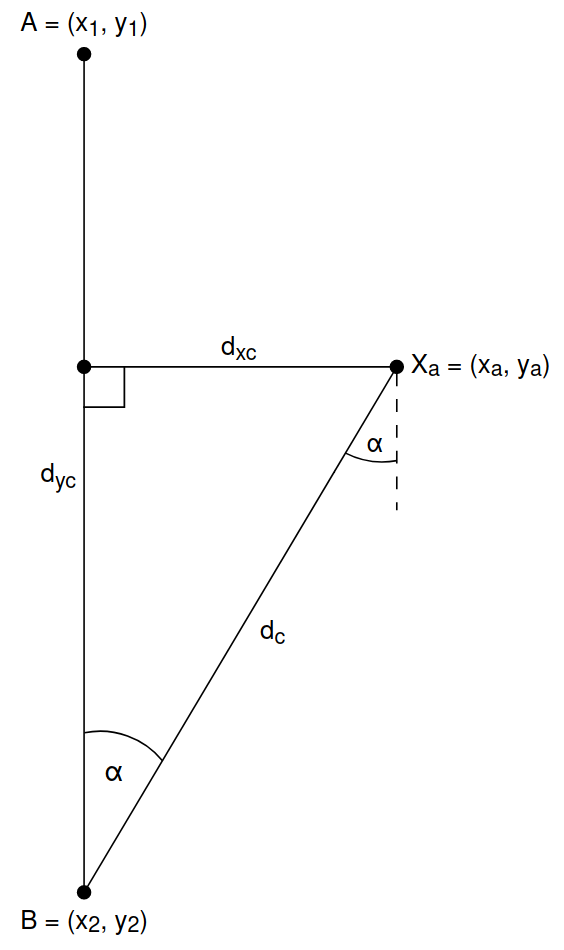
\includegraphics[width=0.65\linewidth]{images/compensacion_vector_distancia_kalman.png}
    \caption{Diagrama de compensación espacial}
    \label{fig:diagcompespacial}
\end{figure}

Para ello podemos definir las expresiones \ref{ec:desplazamiento}, \ref{ec:desplazamiento_x} y \ref{ec:desplazamiento_y}:
\begin{equation}Filtro
    d_c = \sqrt{ {d_{xc}}^2 + {d_{yc}}^2 }
    \label{ec:desplazamiento}
\end{equation}

\begin{equation}
    d_{xc} = x_2 - x_a
    \label{ec:desplazamiento_x}
\end{equation}

\begin{equation}
    d_{yc} = y_2 - y_a
    \label{ec:desplazamiento_y}
\end{equation}

Con lo que podemos calcular $d_c$ para completar la tupla enviada al robot. Ahora bien, en este punto podemos obtener el valor de $\alpha$:

\begin{equation}
    tan(\alpha) = \frac{d_{xc}}{d_{yc}} ; \alpha = arctan(\frac{d_{xc}}{d_{yc}})  
\end{equation}

Es posible comprobar que para un desplazamiento sobre el eje $x$, la diferencia es que se calcula $\alpha$ de la siguiente manera:

\begin{equation}
    \alpha = arctan(\frac{d_{yc}}{d_{xc}})   
\end{equation}

\subsubsection{Compensación vectorial} \mbox{} \vspace{4pt}

Para la compensación vectorial planteamos la situación como en la Figura \ref{fig:diagcompvectorial}, en primera instancia definimos:

$$ V_c = (V_{xc}, V_{yc}) : \text{Vector de compensación} $$

\begin{figure}[htpb]
    \centering
    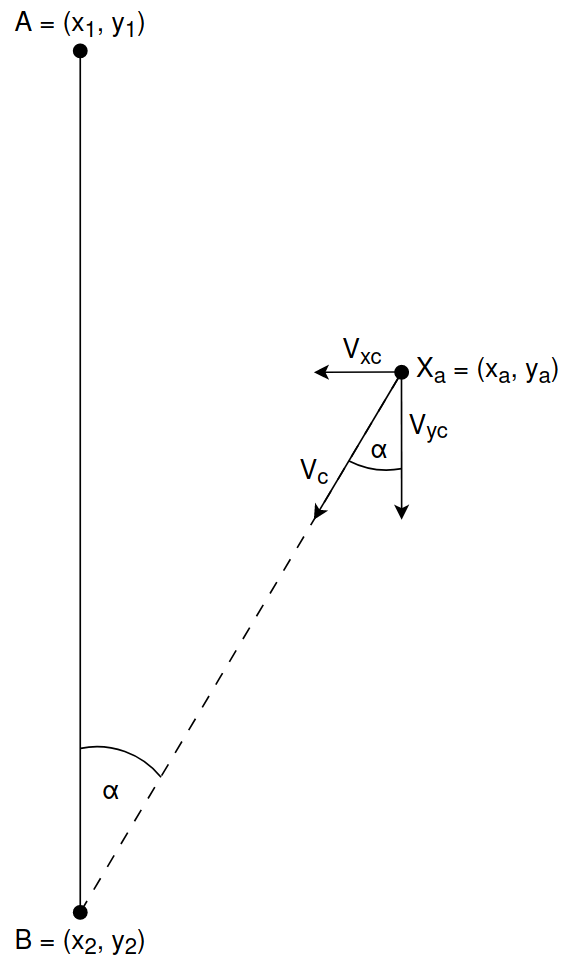
\includegraphics[width=0.65\linewidth]{images/compensacion_vector_velocidad_kalman.png}
    \caption{Diagrama de compensación vectorial}
    \label{fig:diagcompvectorial}
\end{figure}

Ahora bien, se establece que el valor de velocidad de compensación $V_c$ es constante, pero aún así necesitamos descomponer el vector para obtener $V_{xc}$ y $V_{yc}$ para enviarlo al robot:

\begin{equation}
    V_{xc} = V_c \cdot sen(\alpha) 
\end{equation}

\begin{equation}
    V_{yc} = V_c \cdot cos(\alpha)
\end{equation}

Por lo que podemos definir:

\begin{equation}
    tan(\alpha) = \frac{V_{xc}}{V_{yc}} ; \alpha = arctan(\frac{V_{xc}}{V_{yc}})  
\end{equation}

En la tupla del vector de compensación enviado al robot se expresa $v_\theta = 0$ dado que nuestro modelo de Kalman no contempla desplazamiento rotacional.

Es posible comprobar que para un desplazamiento sobre el eje $x$, la diferencia es que calculamos $\alpha$ con la expresión \ref{ec:alpha}:

\begin{equation}
    \alpha = arctan(\frac{V_{yc}}{V_{xc}})
    \label{ec:alpha}
\end{equation}